
\chapter{Real time throughout check}
\label{indexHTML}

By inserting the following script in \texttt{index.html} the browser will
display in real-time the number of pings received by a WebSocket server.

\begin{figure}[H] \centering
  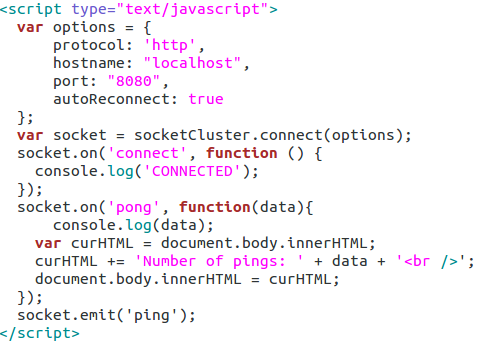
\includegraphics[width=0.8\textwidth]{./Figures/index_script.png}
\caption[Modification to index.html]{Modification to \texttt{index.html}}
\label{fig:index_script} \end{figure}

All it does is emitting a ping, then listening to the pong event and displaying
it directly in the html page. The pong payload as can be seen in
\ref{fig:WS_server_simplePong} is \texttt{count}, an integer incremented each
new ping.

